\section{\label{sec:level1}Experimental Results}
\begin{figure}[b]
\centering
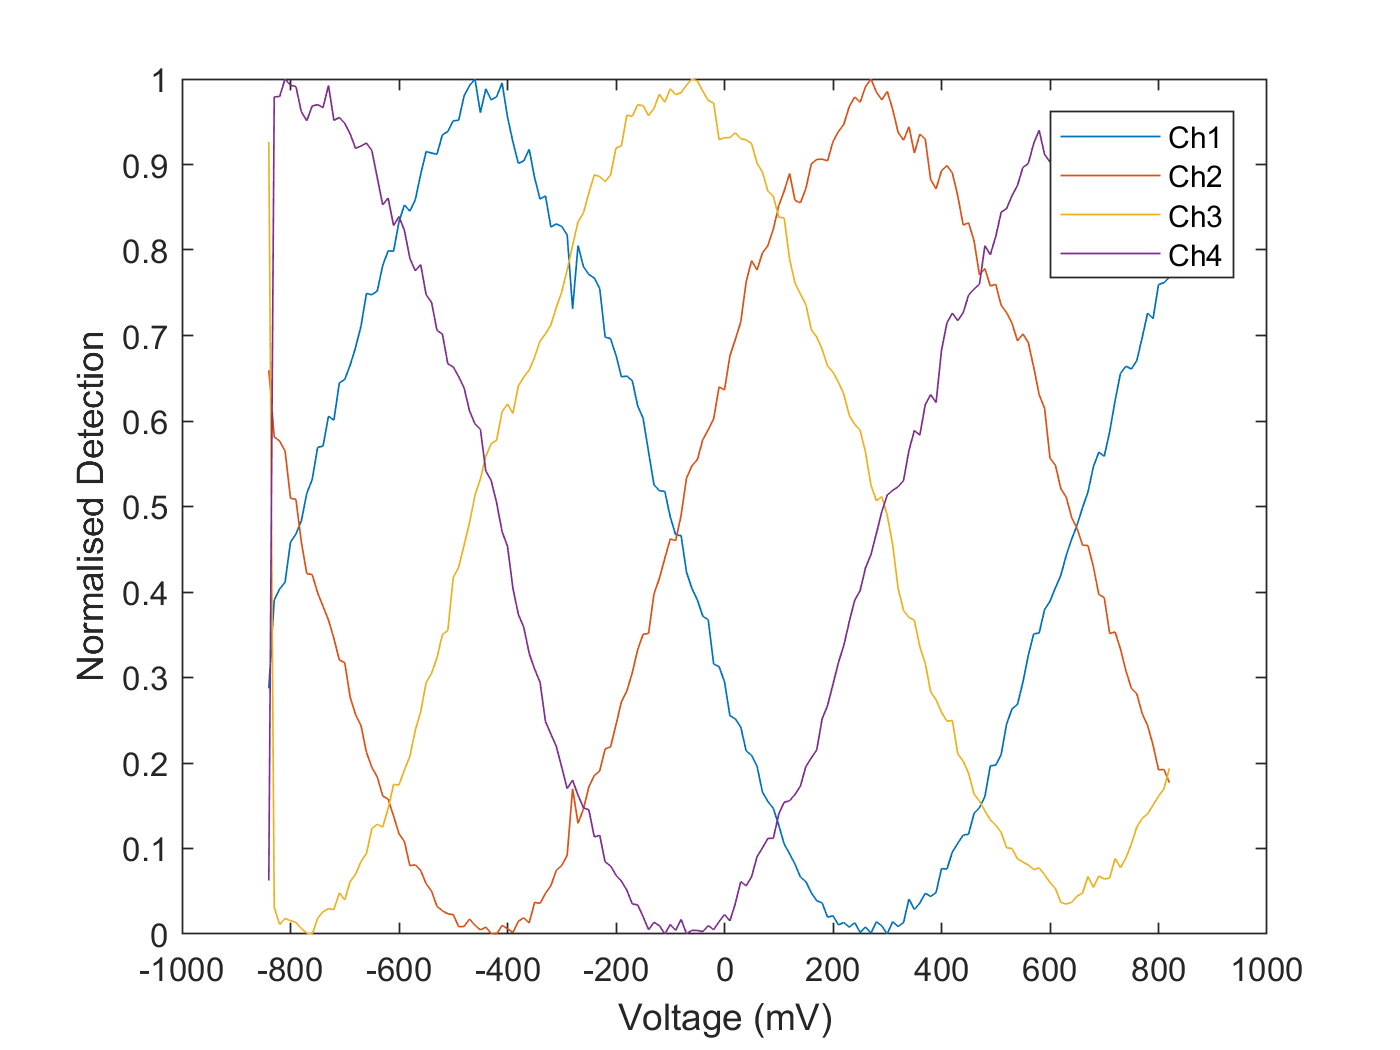
\includegraphics[height=0.33\textwidth,keepaspectratio]{NormalisedEOM}
\caption{\label{fig:NormalisedEOM}The normalised counts as a function of the voltage applied to the EOM amplifier for each detection channel. Channel: Ch1, Ch2, Ch3 and Ch4 measures counts of photons in the polarisation state: $\ket{R},\ket{L},\ket{V},$ and $\ket{H}$, respectively.}
\end{figure}

\begin{figure}[t]
\centering
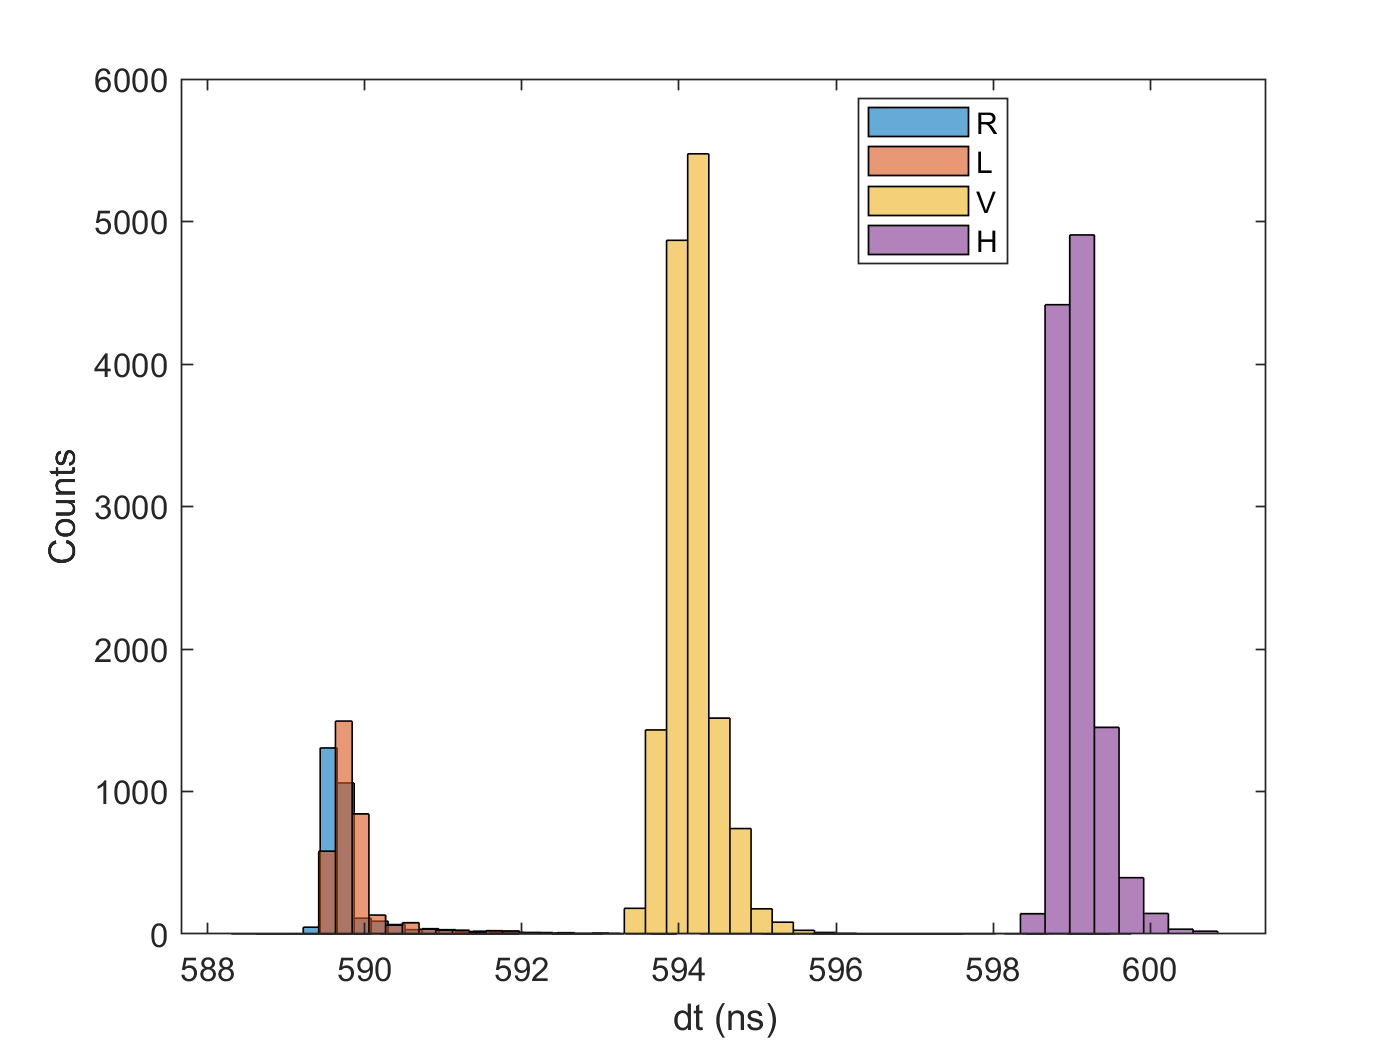
\includegraphics[height=0.33\textwidth,keepaspectratio]{histogramdt}
\caption{\label{fig:histogramdt}The time windowed histogram plot of the counts detected vs. the time between the trigger and the detection event.}
\end{figure} 

\begin{figure}[b]
\centering
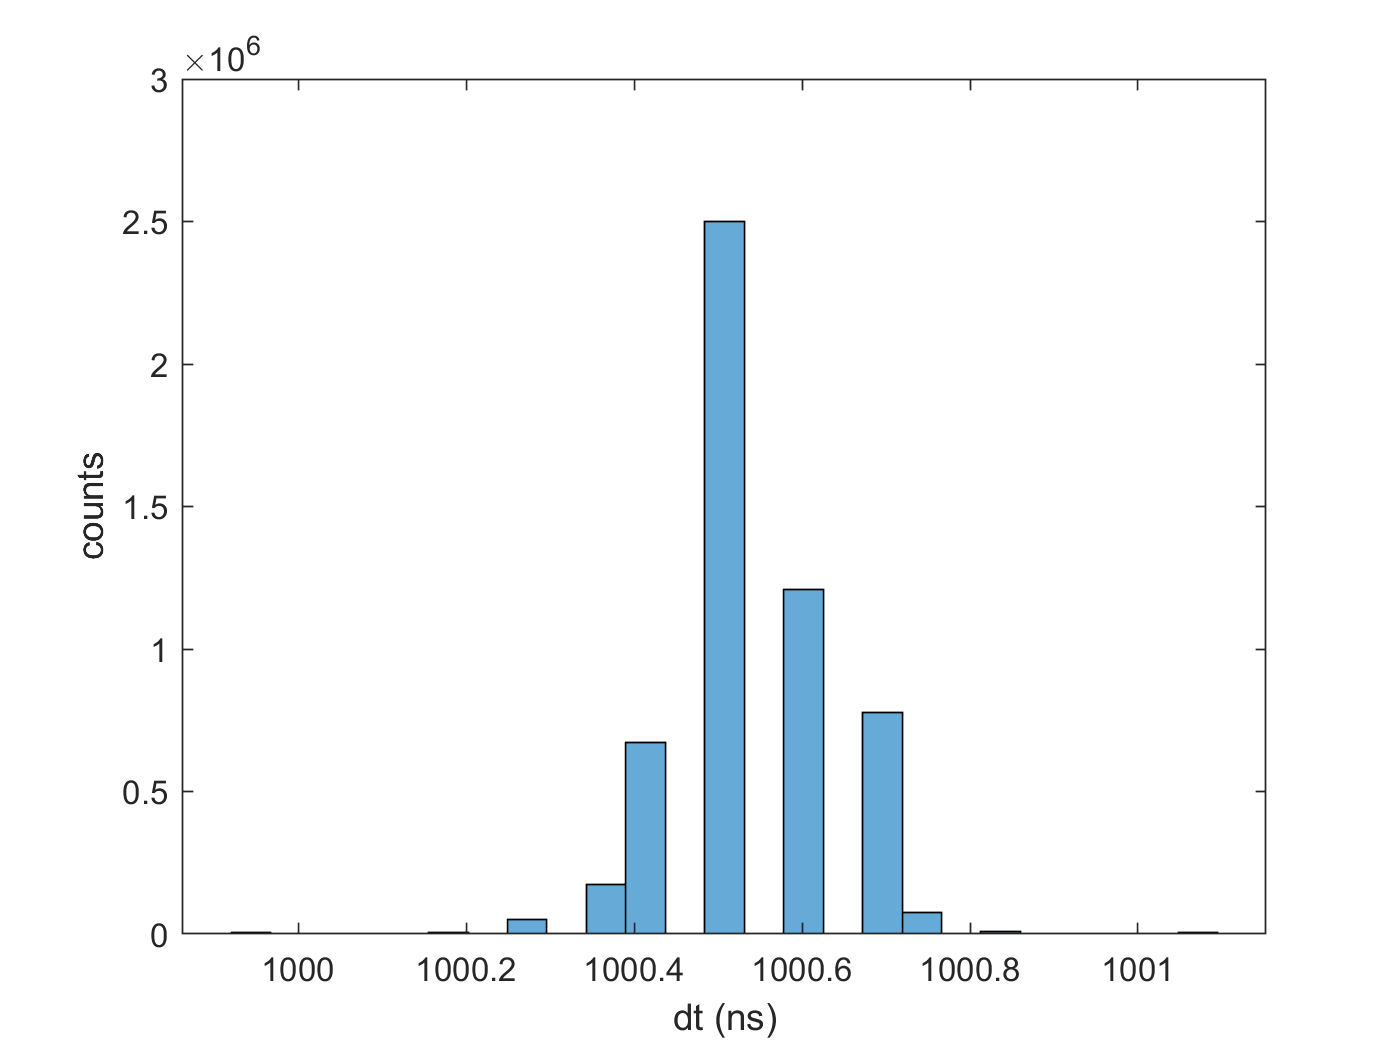
\includegraphics[height=0.33\textwidth,keepaspectratio]{triggerevents}
\caption{\label{fig:triggerevents}Counts vs. time between successive trigger detection events}
\end{figure}

The initial challenge of implementing this scheme is to align the optics shown in Fig. (\ref{fig:opticalsetup}). In particular the laser beam must be efficiently coupled into the fiber optics. To focus the beam into the fiber-couple the distance between the convex coupling lenses was altered in small increments. The DC voltage level was viewed on a oscilloscope by connecting the fiber output to a photon amplifier circuit. Due to the short time available to complete the BB84 experiment, analysis of previously measured data is presented. The ability to transfer a one-time pad with a sufficiency low bit error rate is investigated. 

Initially the small voltage applied $V_{app}$ to the EOM amplifier is swept over a range which will produce all polarisation states. The laser is operated as continuous wave (cw) and the photons are detected by APDs. Since the efficiency of each detector differs, the counts on each channel are rescaled using the data normalisation: $x{}'=(x-x_{max})/(x_{max}-x_{min})$. From the results shown in Fig. (\ref{fig:NormalisedEOM}), it is simple to determine which channel: Ch1, Ch2, Ch3 and Ch4 is connected to the APD which detects photons is the polarisation state: $\ket{R},\ket{L},\ket{V},$ and $\ket{H}$, respectively. The values of $V_{app}$ which correspond to the maximum value of each photon state are obtained to implement the optimum voltage sequence for the one-time pad distribution. 

The photon states sent by Alice, are detected by Bob where $dt$ refers to the difference in time between the trigger detection and the photon detection on a specific channel. The efficiency the APDs results in the difference in the counts across different channels as shown in Fig. (\ref{fig:histogramdt}) where the time window of $dt$ is $(5.88-6.01)\times10^{-7}$ s is chosen to reduce the number of dark counts recorded. The peak position for each histogram varies due to the difference in distance travelled by a single photon to reach each detector. The pulse width of the laser is approximated by calculating the full-width at half maximum (FWHM) from the standard deviation, $\sigma$ of $dt$ for each channel where FWHM = $2\sigma\sqrt{2\ln{2}}$. The average FWHM across the detection channels was 1.18 ns. This is several orders of magnitude larger than the quoted $\approx$ 80 ps pulse width that the laser is operated at. Additionally, the FWHM of for the $dt$ between consecutive trigger detections is calculated as 0.21 ns, this value thus gives the ultimate time resolution of the experiment. 

An estimation of the average photons per pulse is calculated as 0.06 where the individual detector efficiencies are taken as their quoted quantum efficiency. Since detectors are operated as single photon counters there is a dead time after detection reduces the ability to measure the approximately 5 $\%$ two photon occurrence events. Furthermore the dark count rates for the experiment APDs were estimated by initially finding a investigating histogram time binning of $dt$ such that there is a threshold value below which the approximation that any counts are tallied as dark counts is used. The dark count rate of Ch1 and Ch2 are 5.11 Hz and 6.94 Hz are compared to the quoted rate of < 2 Hz. The dark count rate of < 100 Hz is compared to the measured results of 141 Hz and 547 Hz for Ch3 and Ch4 respectively.       

\begin{figure}[t]
\centering
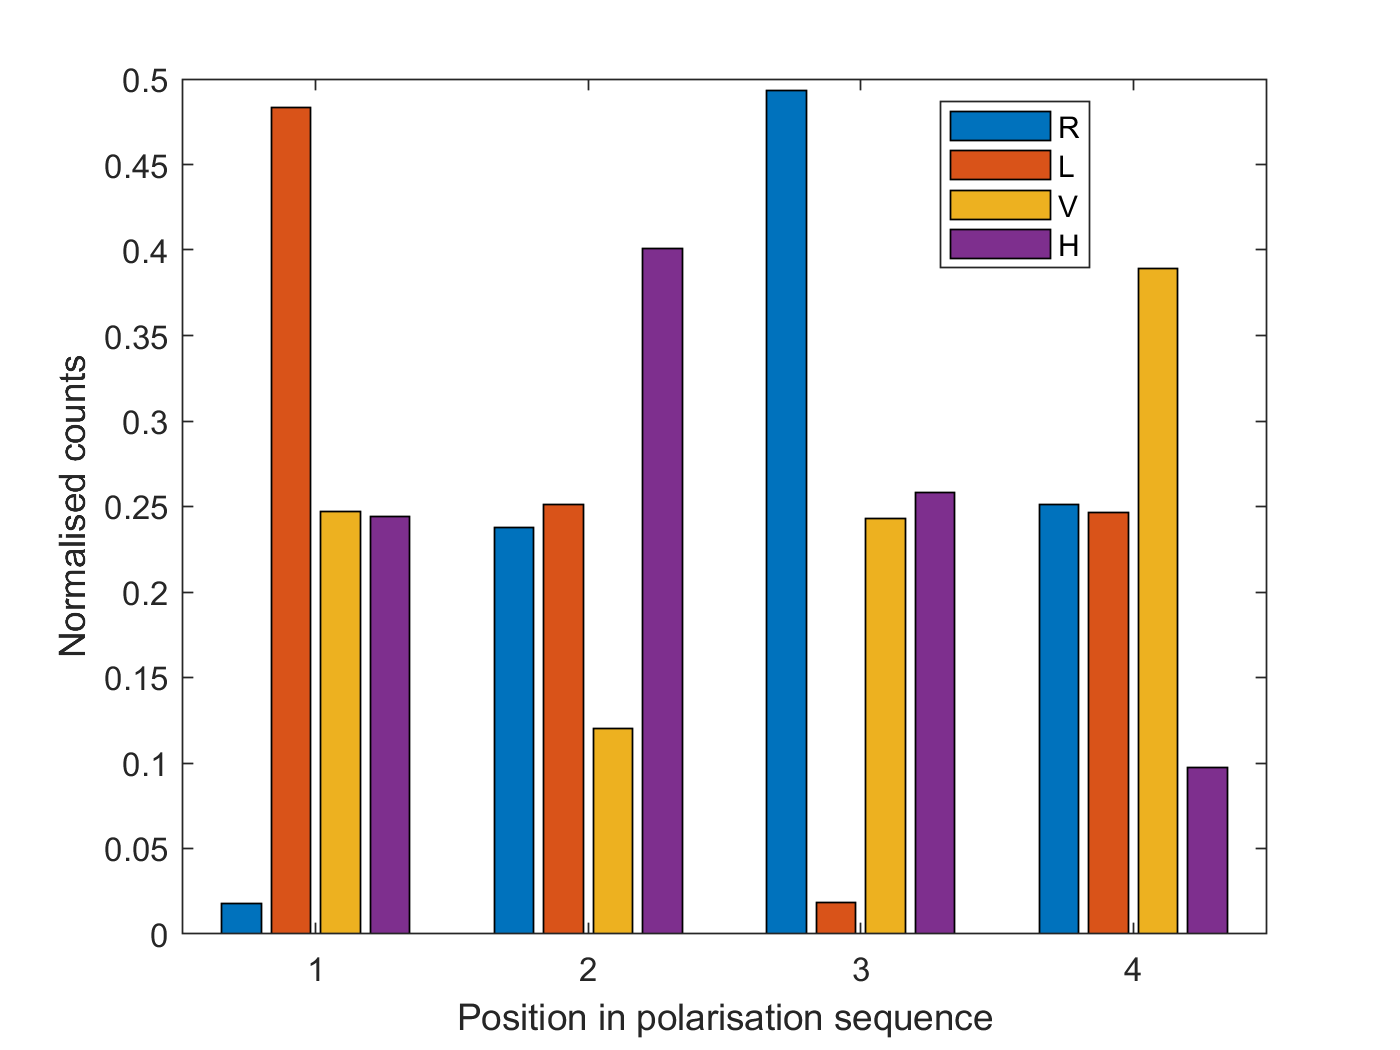
\includegraphics[height=0.33\textwidth,keepaspectratio]{countsvspolarisationstate}
\caption{\label{fig:countsvspolarisationstate}The normalised counts for each detection channel vs. the position in the state preparation sequence. Each colour on the chart corresponds to a different polarisation state detector.}
\end{figure} 

Since the sequence of the $V_{app}$ to the EOM amplifier is repetitive, the number of counts measured on each channel can be determined for the four possible positions in the $V_{app}$ sequence. Here the assumption is made that differences in detector efficiencies can be corrected for as the QKD scheme cannot operate if Bob is biased towards measuring certain states and not others. The normalisation of the counts on each polarisation detector is shown in Fig. (\ref{fig:countsvspolarisationstate}) where the blue bars will sum to 1 etc. From knowing the detectors for each polarisation state detector, the $V_{app}$ sequence prepares the photon states as: $\ket{L},\ket{H},\ket{R},$ and $\ket{V}$, respectively before repeating in this order. The 50 $\%$ probability the polarisation state is measured in the incorrect basis is displayed by the $\approx 1/2$ sum of normalised counts for these polarisation state detectors. This is due to the PBS effectively becoming a 50:50 BS if the photon is polarised in the wrong basis. Alice and Bob can remove these bits from the key string by communicating their prepared and the measurement basis. The QBER which refers to the rate at which errors occur when the data is transmitted is presented for the prepared $\ket{L}$ photon state in position 1. The result is calculated as $R_{1}/(R_{1}+L_{1})$= 3.51 $\%$. Similarly the QBER for the prepared $\ket{H}$, $\ket{R}$ and $\ket{V}$ are given as: 23.1 $\%$, 3.65 $\%$ and 19.9 $\%$, respectively. 



